\chapter{Présentation de la problématique}
    \section{Présentation du sujet}
    Projet avec le laboratoire de \textit{Biologie} de l'\textit{Université des Antilles}, le projet concerne en l'analyse de déplacement de \textbf{Gerridés} afin de déterminer leur préférence sur des zones marquées par des odeurs, en environnement contrôlé.

    \vspace{0.5cm}

    Les \textbf{Gerridés} sont une famille d'insectes de l'ordre des Hémiptères et du sous-ordre des Hétéroptères c'est-à-dire des punaises.
    \begin{figure}[h]
        \centering
        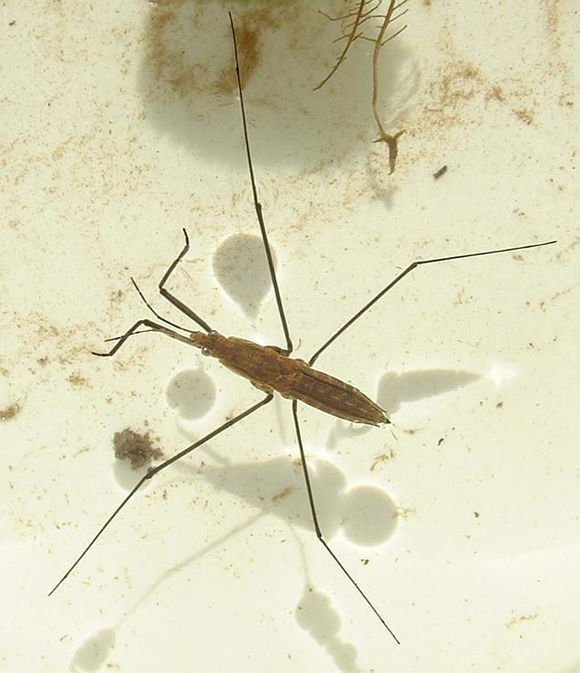
\includegraphics[scale=0.2]{gerrides.jpg}
        \caption{Gérridés}        
    \end{figure}

    \vspace{0.1cm}

    \begin{flushleft}
        Les membres de cette famille sont communément appelés araignées d’eau, mais ce sont des insectes, on ne peut donc pas parler d'araignées. Cette appellation vient sans doute du fait de leurs longues pattes. Leur capacité à se déplacer sur l'eau leur vaut aussi le nom de patineurs de l'eau.        
    \end{flushleft}

    \vspace{0.5cm}

    Afin de déterminer leur préférence, il est nécessaire d'avoir un dispositif adéquat pour leur permettre de se déplacer.
    Ainsi qu'un dispositif de capture vidéo pour l'acquisition de données.

    \vspace{1.6cm}

    \begin{flushleft}
        Le tout étant fait de façon manuelle, les biologistes accrochaient une GoPro au dessus du bac et ensuite devaient la rettirer afin de pouvoir récupérer les données enregistrées. Ce dispositif était très simple à utiliser et leur permettait de réaliser des captures vidéo mais ils leur fallait placé le bac dans le champ de vision de la GoPro a chaque fois qu'ils voulaient faire une capture.\\[0.2cm]
        
        Il fallait aussi que la GoPro soit connecté à un ordinateur afin de pouvoir récupérer les données.\\[0.2cm]

        Ajouter à cela le démarrage et l'arrêt de l'enregistrement de manière manuelle entrainant régulièrement le déplacement du bac (avec les mouvements). La disposition de la GoPro ne permettait de bien voir la prévisualisation de la capture vidéo.\\[0.2cm]

        Les biologistes ont donc décidé d'améliorer leur dispositif afin de pouvoir réaliser l'expérience de manière plus pratique.    
    \end{flushleft}

    \vspace{0.1cm}

    % Pourquoi : Avant c'était fait à la main et c'est pas très efficace.

    \section{Objectifs}
    L'objectifs du stage est de réaliser l'installation et de configurer un dispositif de capture vidéo réalisé par un \textit{Raspberry Pi} ainsi que de développer une application conviviale pour la gestion des vidéos.

    \vspace{0.1cm}

    \begin{flushleft}
        Le dispositif sera installé sur une potence au-dessus du bac et restera fixe en permanence cela limitera les divers déplacements.\\[0.2cm]                
    
        Avec un écran nous pourront interagir avec l'application pour réaliser des captures vidéos.\\[0.2cm]
    
        Le but de cette application est de permettre aux biologistes de réaliser des captures vidéo enregistrées directement sur la carte SD de la Raspberry Pi.\\[0.2cm]

        Et avec un dispositif d'acquisiton de données de manière permanentex.
    \end{flushleft}